\section{Introduction}
Advances in networking, hardware architecture, and programming
languages in recent years have converged to make the choice between
network performance and programmability easier: one can increasingly
afford both.
This has enabled research into hardware implementations of various
applications that were previously confined to software for
programmability or to expensive and inflexible ASICs for performance.

Most prior research in this area has adapted \emph{existing}
applications to run in hardware at line rate.
Example applications include
key-value stores~\cite{Li:2017:KHI:3132747.3132756},
network testing~\cite{Shahbaz:2013:AOS:2537857.2537880},
network stacks~\cite{Istvan:2016:CBI:2930611.2930639},
consensus protocols~\cite{Istvan:2016:CBI:2930611.2930639},
and regex matching on payloads~\cite{Woods:2010:CED:1920841.1920926}.
%and packet filtering~\cite{Fiessler:2016:HVH:2881025.2881033}.

In this paper we describe \OurSys, which to our knowledge is the first application
of its kind. \OurSys is an in-network distributed
mitigation of faulty links.
%We claim that  -- not think necessary - AMD
Our design requires
minimal configuration, is transparent to
end-points and does not conflict
with existing network architecture choices (e.g., the network's topology,
and how packets are routed over it).
We evaluate implementations for CPUs and FPGAs, and model a modified
design using ns-3.


\begin{figure}
  \centering
  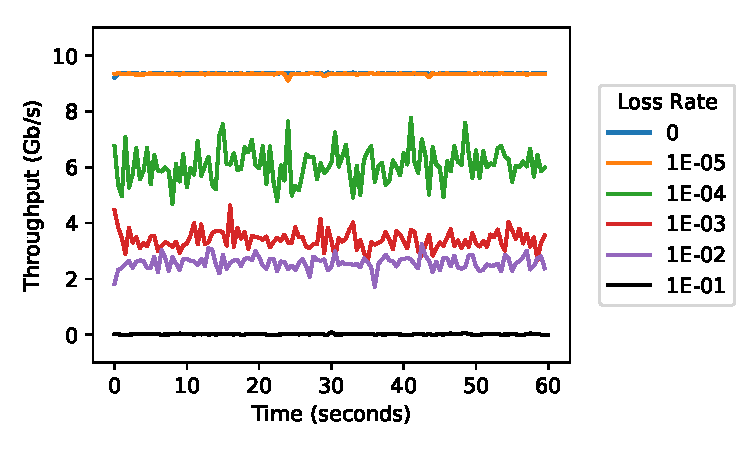
\includegraphics[width=0.3\paperwidth]{figures/timeVsTput.pdf}
  \caption{\label{fig:timeVsTput} Intermittent packet drops at low rates, like those 
  caused by faulty links, drastically reduce TCP throughput.}
\end{figure}


\OurSys can work with various types of networks, but we think it can be
especially helpful in mitigating failing links in datacenters, which has
previously been studied by Zhuo et al.~\cite{Zhuo:2017:UMP:3098822.3098849}.
Datacenter networks are ever more expansive and their architecture involves a
large number of links to attain a larger bisection bandwidth~\cite{Singh:2016:JRD:2991470.2975159}. Their
performance is critical to many widely-used applications, including those
running on private and public clouds. Faulty  links have a significant impact
on these applications, as Figure~\ref{fig:timeVsTput}  illustrates. The
current practice of polling and disabling links from the edge of the network
reacts slowly and adds more contention over non-failing links. \OurSys can help
make such networks more resilient to failing links, with minimal configuration
overhead.

Running \OurSys as an in-network function makes more sense than
running it in end-hosts since the problem that \OurSys mitigates is
typically restricted to a fraction of the network.  Applying \OurSys to
end-hosts adds overhead to all links, also the links that never fail.
%HG: I found the argument that it happens in the network, so we have to fix it
%    there weak.  E.g., TCP flow control also deals with lost packets, a
%    phenomenon that happens in the network, but it is done on the host.
%scoped in the network itself.
%HG: I find the next sentence also a weak argument, candidate for removal.
Just as some application features are
best managed end-to-end~\cite{Saltzer84end-to-endarguments}, handling
link failure seems best done at the link's level. Not only are we able to
identify the faulty link directly, but, unlike higher-layer protocols,
we can also distinguish link failure from congestion.

Programmable network hardware alone is not sufficient to solve this problem: one
also needs a careful design since link management might interfere with
other features of the network, such as topology and routing~
\cite{Greenberg:2011:VSF:1897852.1897877},
%NiranjanMysore:2009:PSF:1594977.1592575,
%Agarwal:2014:SMS:2620728.2620758},
transport~\cite{Raiciu:2011:IDP:2043164.2018467} %,Alizadeh:2010:DCT:1851275.1851192}
and load balancing~\cite{Alizadeh:2014:CDC:2740070.2626316}.
In designing \OurSys, we sought to make it transparent to other
features of the network, to facilitate its interoperation with
existing networks.

Our contributions include (i)~
%the design of \OurSys, which relies on
a link-layer forward error-correction (FEC) scheme to mitigate failing
links, and (ii)~an FPGA implementation of this scheme that fully utilizes 10-Gbps
links. Part of our implementation is in
P4~\cite{Bosshart:2014:PPP:2656877.2656890} over SDNet.
P4's limitation to header processing~\cite{Dang:2017:WPL:3050220.3050231}
was transcended by writing external functions in C for high-level synthesis.
The key challenge we encountered was in streaming packets through our
%It is also a challenge to stream packets through our
external functions.%, and we believe that our approach could be a
%helpful take-away for other researchers. \amd{...but we currently don't
%  deliver on this.}
%  \lei{fixed words}

The next section describes the background and related work of the problem we
are solving, before we describe our design~(\S\ref{sec:design}) and
implementation~(\S\ref{sec:implementation}), which we
evaluate~(\S\ref{sec:evaluation}) before concluding.

%\begin{figure}
%  \centering
%  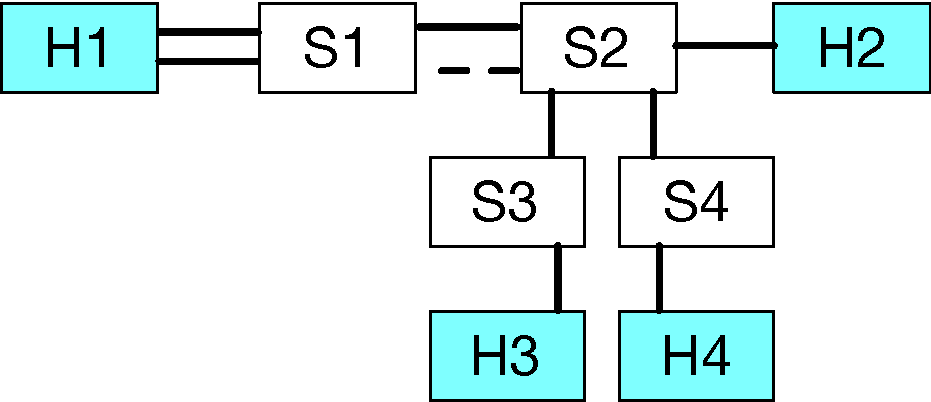
\includegraphics[width=0.3\paperwidth]{example_network.pdf}
%  \caption{\label{fig:example-net}An example network consisting of four
%    switches (S1-S4) and four hosts (H1-H4). Faulty links are shown as dashed lines.
%    Each link is assumed to have capacity $R$ unless the link is faulty, in
%    which case it has capacity $F < R$.  In this example, the failing link
%    diminishes the bandwidth of H1.}
%\end{figure}
